\chapter{Feedline Design}
In \cref{study-focus}, we outlined the focus of this thesis, which is to investigate the factors which affect
the transmission we get from the feedline. In particular, we will focus on the geometric properties of the
feedline, and investigate how different features in the geometry affect its transmission. We will do that in
\cref{results}, but before that it will be useful to go over some basic theory of the feedline structure,
which we will do in this chapter. 

\section{Theory}
\label{cpw-theory}
\begin{figure}
	\centering
	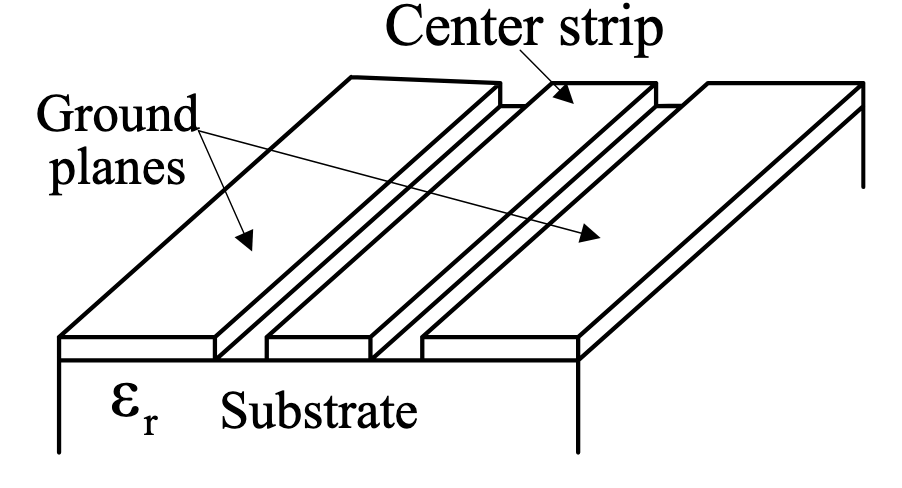
\includegraphics[scale=0.5]{images/cpw-diagram.png}
	\caption{General geometry of a coplanar waveguide. Notice that the planes on either end are set to
		ground, and the center strip is set to a voltage \( V(t, z) \). All three strips lie on the substrate \(
	\epsilon_r \). This diagram is taken from \cite{gaoPhysicsSuperconductingMicrowave}.}  
	\label{cpw-diagram}
\end{figure}

For this section, we will largely follow the derivation provided in
\cite{gaoPhysicsSuperconductingMicrowave}, specifically sections 3.1.1 and 3.1.2. For a more thorough
explanation, we refer to the remaining chapters in \cite{gaoPhysicsSuperconductingMicrowave}.
The basic structure of the feedline is called a coplanar waveguide (CPW). A diagram of its basic geometry
is shown in \cref{cpw-diagram}: it is characterized by having three metal strips placed on top of a substrate
layer of permittivity \( \epsilon_r \), with the two outer strips being grounded and the center being the
signal strip. In the general case of a wave propagating through a waveguide, one may write the \( \mathbf{E}
\) and \( \mathbf{B} \) fields generally as:
\[
	\mathbf{X}(x, y, z) = [\mathbf{x}_t(x, y) + x_z(x, y) \mathbf{\hat{z}}] e^{-j \beta z}
\]
Here, \( \mathbf{X} \) is a general vector field that represents both the electric field \( \mathbf{E} \) and
auxiliary field \( \mathbf{H} \). In other words, we can decompose the vector field into its transverse and 
longitudinal (\( \mathbf{\hat{z}} \)) components; this is
fine because both components are linearly independent. To find how waves propagate in a CPW, the standard
approach is the same as we use for any waveguide: we just solve Maxwell's equations to see which solutions
the CPW configuration admits. 
In the case where the metal strips are perfect conductors and we submerge the CPW in a homogeneous medium
(i.e. we the entire space is filled with a substrate of permittivity \( \epsilon_r \)), then the solutions
to Maxwell's equations indicate the presence of a pure TEM mode. This mode can essentially be understood as a
perfect standing wave, where the longitudinal (i.e. \( \mathbf{\hat{z}} \) direction) component of \(
\mathbf{E} \) and \( \mathbf{H} \) are zero and the transverse current density \( \mathbf{J} \) also goes to
zero.

However, the case in any realistic CPW is not so simple: as indicated by \cref{cpw-diagram}, the space in
which the CPW exists does not have uniform \( \epsilon_r \), and secondly, the metal strips have finite
conductivity, and are thus not perfect conductors. These two factors combined makes the pure TEM mode
impossible with our superconducting CPW. However, as outlined in \cite{gaoPhysicsSuperconductingMicrowave}, a
superconducting CPW gets \textit{close enough} to a pure TEM mode, in that the non-TEM component of the wave
remains small. For this reason, we say that the CPW admits a quasi-TEM mode -- in essence, we are able to use
the theoretical results that come with the pure TEM without worrying too much because the non-TEM effects are
negligible.         
 
\subsection{Impedance}
One characteristic of the CPW we must pay close attention to is its impedance. This is particularly so
because in an ideal world, we want a constant impedance throughout the feedline, so as to minimize
distortions to the signal that we send into the detector, and be able to impedance match to our start and end
ports. Thus, it pays to spend some time discussing the factors that govern the impedance of our CPW. 

To do so, we first identify that the CPW has a characteristic impedance and capacitance, denoted \( L \) and
\( C \). Its characteristic impedance is calculated as \( Z_0 = \sqrt{L / C} \), hence the only two
quantities that we need to calculate are \( L \) and \( C \) themselves. As mentioned at the 
end of \cref{cpw-theory}, because we can approximate the field solution as a TEM mode (i.e. standing wave), 
this means that the transverse electric field \( \mathbf{e}_t \) and auxiliary field \( \mathbf{h}_t \) can 
be analytically solved by considering it as a two-dimensional statics problem.

First, we tackle the case of the electric field \( \mathbf{e}_t \) over all space. 
To begin, because we are dealing with a superconductor, it is sufficient to make the argument that we are
dealing with an approximately perfect conductor -- this means that we can assume \( \mathbf{e}_t \) inside
the superconductor to be zero, and \( \mathbf{e}_t \) outside the superconductor to be approximately equal to
the case of a perfect conductor. Because there are no charges outside the superconductor, it follows that the
electric potential outside the superconductor satisfies Laplace's equation:
\[
	\nabla^2 \Phi = 0
\]
which we can then back out the electric field using \( \mathbf{e}_t = \nabla \Phi \). From here, we can
calculate the capacitance \( C \), which we detail how to do in \cref{conformal-map}. For the magnetic field,
we can make a similar assumption, approximating the superconductor as a perfect conductor. Doing this, we
conclude that the vector potential \( A_z(x, y) \) is constant within the superconductor, and outside the
superconductor it also satisfies Laplace's equation:
\[
	\nabla^2 A_z = 0
\]
Now that we have the setup, how do we actually go about solving such equations? To do this, one common
technique involves using a conformal mapping, which we will detail in the section below.      

\subsection{Conformal Mapping}
\label{conformal-map}
Conformal mapping is a popular and powerful technique to solving such two-dimensional static problems. In
particular, consider the two-dimensional Laplace's equation we ultimately wish to solve:
\[
	\pdv[2]{\Phi}{u} + \pdv[2]{\Phi}{v} = 0
\]
The solution to any complex differential equation is a function of the form \( z = f(w) \), which can be
understood as a function which maps one coordinate \( (u, v) \) to a new coordinate \( (x,y) \). Complex
analysis now gives us a very powerful tool: if \( f \) is analytic and is also one-to-one, then it follows
that Laplace's equation is invariant under \( f \), so we can pick any other domain \( (x, y) \) 
to solve over so long as it is related to the original \( (u, v) \) by an appropriate \( f \). Essentially, 
what this property allows us to do is solve Laplace's equation in an easier domain \( (x, y) \), which then 
also solves the equation in the original \( (u, v) \) domain via \( f \). 

One particular \( f \) that is useful to us is called the Schwarz-Christoffel mapping. Without going into too
much detail, the function \( f \) is expressed as:
\begin{equation}
	\label{sc-map}
	 z = f(w) = f(w_0)  + c \int_{w_0}^{w} \prod_{j = 1}^{n - 1}(w' - w_j)^{\alpha_j - 1} \diff w'
 \end{equation}
This mapping essentially turns a closed polygon and "straightens" it out,
mapping it to the upper half complex plane. Our CPW can be easily modeled as a closed polygon, so this is
indeed an appropriate mapping to choose. Then, as described, we solve Laplace's equation in the upper half
plane, and use \( f \) to map that solution back onto our CPW. 
 
For our particular CPW, it's thin enough that it can be approximated by a geometry with zero thickness, which
is beneficial to us because it makes the mathematics significantly easier. 
This process is summarized in \cref{cpw-conformal}, showing how the conformal mapping of the CPW changes its
geometry into one that is more desirable on the right, from which it is easier to calculate the capacitance.
The quantity \( K \) and \( K' \) denote the width of the lower and upper CPWs after the transformation,
which are calculated using elliptical integrals: 

\begin{align*}
	K = K(k) &= \int_{0}^{1}\frac{1}{\sqrt{(1 - x^2)(1 - k^2 x^2)}} \diff x\\
	K' = K(k') &= \int_{1}^{1 / k} \frac{1}{\sqrt{(x^2 - 1)(1 - k^2 x^2)}} \diff x
\end{align*}

\begin{figure}
	\centering
	\begin{subfigure}{0.4\textwidth}
		\begin{tikzpicture}
			\draw (-3, 0) -- (3, 0) node[right] {\( u \)};
			\draw[-stealth] (0, -1) -- (0, 2) node[above] {\( jv \)};

			\draw[very thick, stealth-] (-3, 0) node[above] {\tiny \( -\infty \)} -- (-2, 0) node[below] {\( -b \)};
			\draw[very thick] (-1, 0) node[below] {\( -a \)} -- (1, 0) node[below] {\( a \)};
			\draw[very thick, -stealth] (2, 0) node[below] {\( b \)} -- (3, 0) node[above] {\tiny \( \infty \) };
		\end{tikzpicture}
		\caption{}
		\label{conformal-1}
	\end{subfigure}
	\hspace{2cm}
	\begin{subfigure}{0.4\textwidth}
		\begin{tikzpicture}
			\draw (-3, 0) -- (3, 0) node[right] {\( \sigma \)};
			\draw[-stealth] (0, -1) -- (0, 2) node[above] {\( j \eta \)};
			\draw[very thick] (-1, 0) node[below] {\( -K \)} -- (1, 0) node[below] {\( K \)};
			\draw[very thick] (-1, 1) -- (0, 1) node[above right] {\( jK' \)} node[below left]
				{\tiny \( -\infty \)} node[below right] {\tiny \( \infty \)} -- (1, 1);
			\draw (-1, 0) -- (-1, 1);
			\draw (1, 0) -- (1, 1);
		\end{tikzpicture}
		\caption{}
		\label{conformal-2}
	\end{subfigure}
	\caption{Conformal mapping of coplanar waveguide with zero thickness using the SC-mapping. (a) The
		original diagram for the CPW. (b) The shape of the CPW after the conformal mapping. The "ground"
		strips are assumed to be infinite; notice how they "bend" into the shape of a rectangle. This figure is
	taken from \cite{gaoPhysicsSuperconductingMicrowave}, reproduced here by for clarity.}          
	\label{cpw-conformal}
\end{figure}

Here \( k = a / b \) is a ratio determined by the gap between the center and ground lines, and \( k' =
\sqrt{1 - k^2} \). The exact means by which we derive this formula is not important at the moment, but what
is important is that these two quantities, \( K(k) \) and \( K(k') \) directly relate to the capacitance and
inductance:
\[
	C =\frac{1 + \epsilon_r}{2} \epsilon_0 \frac{4K(k)}{K(k')} \quad L = \mu_0 \frac{K(k')}{4K(k)}
\]
The key insight in this equation is \( C \) and \( L \), and thus \( Z_0 = \sqrt{L / C} \), depends
\textit{solely} on two quantities: the gap width and the relative permittivity of the substrate given by \(
\epsilon_r \). So, in theory, what this means is that as long as we don't change the ratio \( a / b \)
and keep the substrate the same throughout the system, the impedance of the CPW should remain constant.

\section{Simulation Setup}
\label{setup}

\begin{figure}
	\centering
	\begin{subfigure}{0.4\textwidth}
		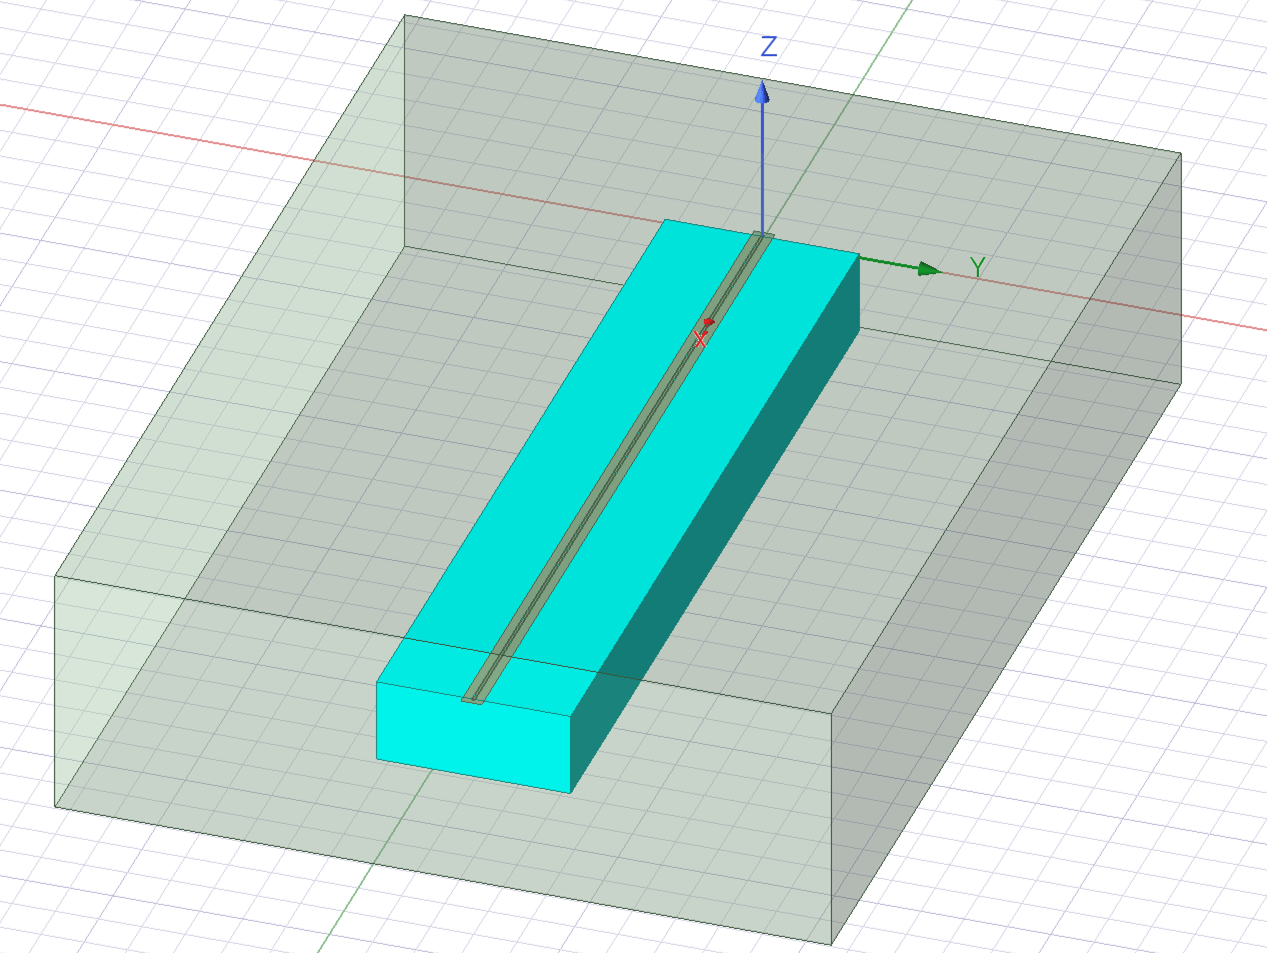
\includegraphics[scale=0.15]{images/short-finiteconductivity.png}
		\caption{}
		\label{short-model}
	\end{subfigure}
	\hspace{0.5cm}
	\begin{subfigure}{0.4\textwidth}
		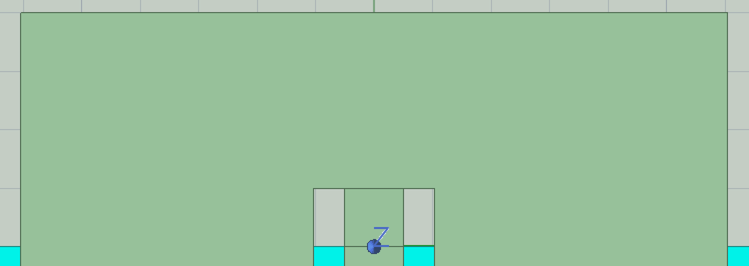
\includegraphics[scale=0.3]{images/port-geometry.png}
		\caption{}
		\label{port-geometry}
	\end{subfigure}
	\caption{(a) Screenshot showing one of the simulation models we performed. The silicon substrate is
		colored in blue, with the CPW sitting on its surface. The entire apparatus is enclosed in a
	conducting box. (b) Close-up screenshot of one of the lumped port excitations in the simulation. The
	lumped port is the small rectangle in the middle, which is surrounded by the center line just below it
	and the ground lines connected to it from above. Notice that the ground lines are connected together,
	this is just to ensure that they are both at the same voltage. } 
\end{figure}

Here, we discuss the setup of the CPW simulations that were performed. The simulations were completed in
Ansys HFSS, a high-precision finite element analysis (FEA) software that specializes in RF simulations.
\cref{short-model} shows a typical example of a model that was simulated. In each simulation, we
use a CPW with a central line of width of 20 microns, and ground lines of width 100 microns. The gap between
was calibrated to 10.75 microns. The substrate is silicon, with a relative permittivity of 11.9. 
Given these specifications, we used a calculator provided by 
\href{https://www.microwaves101.com/calculators/864-coplanar-waveguide-calculator}{this link} to determine
the impedance \( Z_0 \), which comes out to about 50 ohms. We also enclose the entire waveguide inside of a
conducting box -- this is also for experimental reasons, as current prototypes for KIDs are built with a
similar box around them. 

As mentioned, the focus with this thesis is that the impedance of our waveguide remains constant from end to
end. Further, we explored at the end of \cref{conformal-map} that this condition can be guaranteed, at least
in theory, when we don't change the ratio \( k = a / b \) throughout the length of the waveguide.
The specific reason we chose 50 Ohms is to be consistent with existing experimental setups,
but in principle this number can be altered and it wouldn't matter very much for the focus of this
investigation.   

One detail that should be mentioned is that in \cref{conformal-map}, we assumed the ground lines to be
infinitely long, as shown in \cref{conformal-1}, yet this is obviously impossible with physical simulations. However,
recall that the only thing we need to ensure is that the gap remains constant, so the width of the ground
strips don't matter very much, as long as we make them long enough. In our case, the width of the ground
strip is roughly ten times times larger than that of the central line, 
which is large enough that making the ground strip larger would not make a large difference to 
the overall impedance.    

The simulation is excited by two lumped ports with impedance set to 50 ohms, labeled ports 1 and 2, placed at
either end of the waveguide. These ports are responsible for sending the input signal into the waveguide,
which we set to frequencies between 1GHz and 10GHz. This specific frequency range was selected since 
these ports are placed so that they don't touch the substrate material but are
in contact with the center and ground planes, via the geometry shown in \cref{port-geometry}. As shown, the
lumped port hangs off the side of the substrate, which is important because the port is already calibrated to
an impedance of 50 ohms; the presence of the substrate could alter this value, leading to impedance mismatch.

\subsection{Voltage Standing Wave Ratio (VSWR)}
\label{swr}
The Voltage Standing Wave Ratio (VSWR) is the particular quantity that we calculate in our simulations which characterizes
the transmission quality of our CPW. It is a common measurement quantity in RF simulations, as it is a
measurement giving us information about how well the impedance matching in our system is. At its core, the
VSWR is calculated as:
\[
	\text{VSWR} = \frac{|V_\text{max}|}{|V_\text{min}|} = \frac{1 + |\Gamma|}{1 - |\Gamma|}
\]
Here, \( \Gamma \) is called the \textit{reflection coefficient}, expressed as:
\[
	\Gamma = \frac{V_r}{V_f}
\]
Due to the nature of the absolute value in the calculation for VSWR, its range of values is between 1 and
infinity. When the value of \( \Gamma \) is zero, this leads to a VSWR value of 1, which therefore
corresponds to no reflection (alternatively, perfect transmission). On the other hand, the larger the VSWR
value is, more of the wave is said to be reflected as \( |\Gamma| \) is larger. In practice, \( \Gamma \) is
a complex number that also encodes the phase of the reflected wave, but for our purposes we only care about
the magnitude.   


 
 
 
